\begin{figure}[H]
\scalebox{0.5}{%
    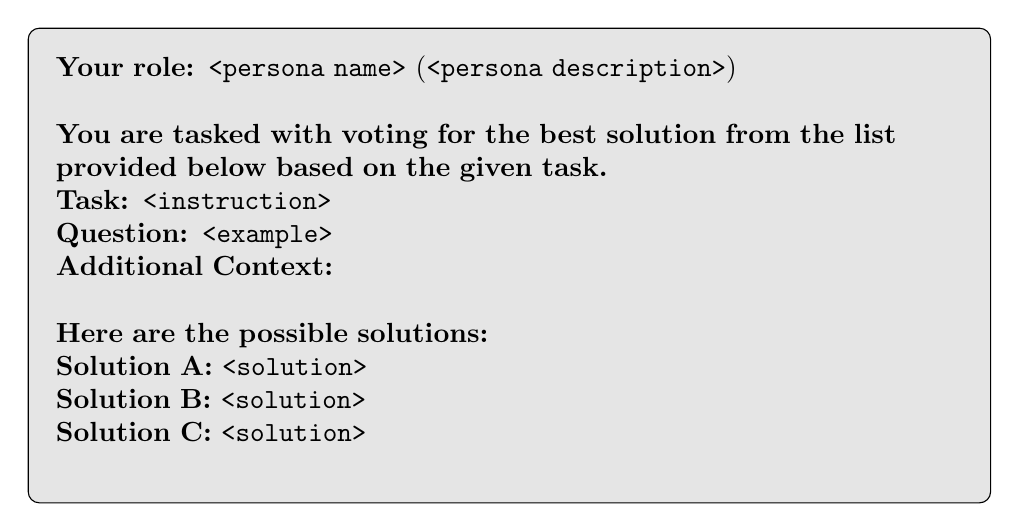
\begin{tikzpicture}
    \node [draw, rectangle, rounded corners, fill=gray!20, text width=0.95\textwidth, inner sep=10pt] (block) {
        \begin{minipage}{\textwidth}
        \textbf{Your role:} \texttt{<persona name>} (\texttt{<persona description>}) \\
        
        \textbf{You are tasked with voting for the best solution from the list provided below based on the given task.} \\
        \textbf{Task:} \texttt{<instruction>} \\
        \textbf{Question:} \texttt{<example>} \\
        \textbf{Additional Context: } \\

        \textbf{Here are the possible solutions:} \\
        \textbf{Solution A:} \texttt{<solution>} \\
        \textbf{Solution B:} \texttt{<solution>} \\
        \textbf{Solution C:} \texttt{<solution>} \\
        \end{minipage}
    };
    \end{tikzpicture}
}
\caption{Prompt to process the voting at the end of each turn. The number of solutions to vote for can vary depending on the proposals made by the agents.}
\end{figure}
